\documentclass{article}

% Language setting
% Replace `english' with e.g. `spanish' to change the document language
\usepackage[english]{babel}
\usepackage{amsfonts}
\nocite{*}

% Set page size and margins
% Replace `letterpaper' with `a4paper' for UK/EU standard size
\usepackage[letterpaper,top=2cm,bottom=2cm,left=3cm,right=3cm,marginparwidth=1.75cm]{geometry}

% Useful packages
\usepackage{amsmath}
\usepackage{graphicx}
\usepackage[colorlinks=true, allcolors=blue]{hyperref}

\title{%
Research Assignment\\
\vspace{0.5cm}
  \textbf{Fuzzy Arithmetic on Gaussian Fuzzy Number}\\
  \large 
  \vspace{0.8cm}
  Course : BITS F343 Fuzzy Logic and Applications\\
  \vspace{0.1cm}
  Instructor: Dr. Chandra Shekhar 
  \vspace{0.5cm}
  }
\author{
  Anish Kulkarni\\
  \texttt{2020A7PS0975P}
  \and
  P V S Tarak Shree Vallabha\\
  \texttt{2020A7PS1513P}
  \and
  Dr. Chandra Shekhar\\
  \texttt{csbits.fuzzy@gmail.com}
\vspace{0.6cm}
}

\date{December 10, 2022}
\begin{document}
\maketitle

\begin{abstract}
Arithmetic operations like addition, subtraction, multiplication, division on the Gaussian Fuzzy Number are discussed in the document. Exponentiation and Logarithm are also discussed briefly.
\end{abstract}

\section{Introduction}
Fuzzy numbers are a special type of fuzzy set. There exist different types of fuzzy numbers like, triangular fuzzy number, trapezoidal fuzzy number, pentagonal fuzzy number, L-R fuzzy numbers etc. One of these types if the Gaussian Fuzzy Number. The document begins with an introduction of the preliminaries that we require to understand the Gaussian Fuzzy Number and any operations performed on it.

\section{Preliminaries}

\subsection{Fuzzy Set}

Consider a non-empty Crisp set $X$. A fuzzy set $\Tilde{A}$ on set $X$ is defined as follows:
\begin{equation}
    \Tilde{A} = \{ \: (x, \mu_{\Tilde{A}}(x)) \: : \: x\in{X}, \: \mu_{\Tilde{A}} : X\to{[0,1]} \: \}, 
\end{equation}
where $\mu_{\Tilde{A}}$ is called the membership function of the $\Tilde{A}$  and set $X$ is called the universe of discourse of $\Tilde{A}$.

\subsection{Normal Fuzzy Set}

 Consider a fuzzy set $\Tilde{A}$ with universe of discourse $X$. $\Tilde{A}$ is said to be a normal fuzzy set if there exist at least one $x \: \in X $ such that $\mu_{\Tilde{A}}\:=\:1$.

 \subsection{Support of a Fuzzy Set}
Consider a fuzzy set $\Tilde{A}$ with universe of discourse $X$. The support of $\Tilde{A}$ denoted by $Supp(\Tilde{A})$ is a crisp set given by :
\begin{equation}
    Supp(\Tilde{A}) = \{ \: x \: : \: x \in {X} ,\: \mu_{\Tilde{A}}(x) \: > 0 \: \}
\end{equation}

\subsection{$\alpha$-cut a Fuzzy set}
For a fuzzy set $\Tilde{A}$ defined on $X$, the $\alpha$-cut of $\Tilde{A}$ for $\alpha \in [0,1]$, denoted by $\Tilde{A}_\alpha$ is a crisp set defined as:
\begin{equation}
    \Tilde{A}_{\alpha} = \{ \: x \: : x\in{X}, \: \mu_{\Tilde{A}}(x) \geq \alpha \: \}
\end{equation}

\subsection{Fuzzy Number}
A fuzzy set $\Tilde{A}$ defined on $\mathbb{R}$ is said to be a fuzzy number if it has the following properties:
\begin{enumerate}
    \item $\Tilde{A}$ must be a normal fuzzy set.
    \item $\Tilde{A}_\alpha$ must be closed for every $\alpha \in [0,1]$.
    \item The support of $\Tilde{A}$, $Supp(\Tilde{A})$ must be bounded.
\end{enumerate}

\subsection{Gaussian Distribution}
Gaussian Distribution, also known as Normal Distribution is a continuous probability distribution for a real-valued random variable. The probability density function of a Gaussian Distribution is given by:
\begin{equation}
    \mathcal{N}(\mu , \sigma{^2}) = \frac{1}{\sigma \sqrt{2\pi}}e^{-\frac{1}{2}(\frac{x-\mu}{\sigma})^2}
\end{equation}
where $\mu \in \mathbb{R}$ and $\sigma{^2}\in\mathbb{R}^{+}$ represent the mean and variance of the Gaussian probability distribution on $x\in\mathbb{R}$. Gaussian distribution is sometimes informally called a bell-shaped curve. Figure \ref{fig:gauss} shows a Gaussian distribution with $\mu = 50$ and $\sigma = 10$.

\begin{figure}
    \centering
    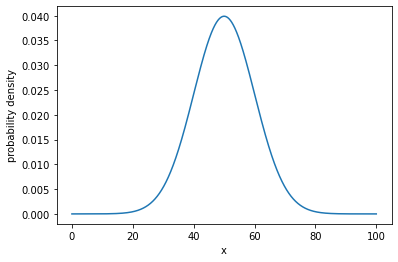
\includegraphics[scale=0.5]{gaussian_dist.png}
    \caption{\label{fig:gauss} Gaussian distribution with $\mu = 50$ and $\sigma = 10$. }
    \label{fig:gauss}
\end{figure}

\subsection{Gaussian Fuzzy Number}
The membership function of a Gaussian fuzzy number $\Tilde{A}$ on $\mathbb{R}$ is given by:
\begin{equation}
    \mu_ {\Tilde{A}} (x) = e^{\left[ \frac{-(x-m)^2}{2\sigma^{2}} \right]} \: \forall {x} \in \mathbb{R}, \: \sigma > 0,\; m\in \mathbb{R}
\end{equation}
Figure \ref{fig:gaussno} shows Matlab plot for a Gaussian Fuzzy number with $\mu = 20$ and $\sigma = 5$.

\begin{figure}
    \centering
    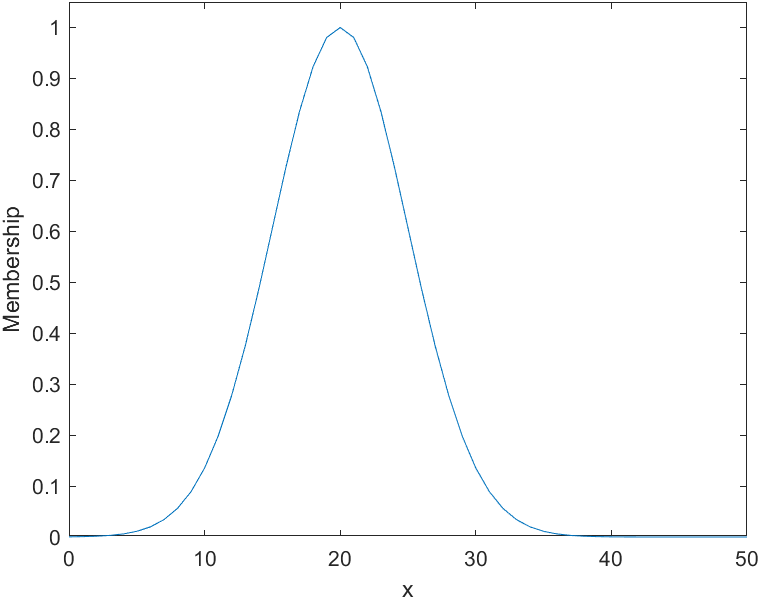
\includegraphics[scale=0.6]{gaussno.png}
    \caption{\label{fig:gaussno} Gaussian Fuzzy Number with $\mu = 20$ and $\sigma = 5$}
    \label{fig:gaussno}
\end{figure}

\subsection{L-R Representation of a Fuzzy number}
In the L-R representation of a fuzzy number, $\Tilde{P}$ is represented by :
\[ \Tilde{P} \:=\: \left( m, \alpha, \beta\right)_{L,R} \] \newline Here, m represents the modal value of the membership function, $\alpha$ and $\beta$ represent the left-spread and the right-spread of the membership curve respectively, and $L$ and $R$ represent the left and right shape functions of the membership curve of $\Tilde{P}$. The membership function of an L-R fuzzy number, $\Tilde{P}$ is given by:
\begin{equation}
    \Tilde{P} \:=\: \left( m, \alpha, \beta\right)_{L,R} = \begin{cases}
        L\left(\frac{m-x}{\alpha} \right) & \text{if } x \leq m\\
        R\left(\frac{x-m}{\beta} \right) & \text{if } x > m
    \end{cases}
\end{equation} \newline The $\alpha$-cut for an L-R fuzzy number $\Tilde{P} = \left( m, p, q\right)_{L,R}$ is given by:
\begin{equation} \label{alpha_lr}
     \Tilde{P}_\alpha \:=\: \left[ m - p L^{-1}(\alpha),  m + q R^{-1}(\alpha) \right]
\end{equation} \newline For a Gaussian fuzzy number $\Tilde{A}$ with mean $m$ and standard deviation $\sigma$, 
\begin{equation}
   L(u) = R(u) = e^{\frac{-u^2}{2}}\:, \: \Tilde{A}\,=\,(m, \sigma, \sigma)_{L,R} 
\end{equation}

\subsection{Tangent and Secant Approximations}
To simplify calculation of result during multiplication, reciprocal, and division of L-R fuzzy numbers, two approximations were proposed, namely \textit{Tangent Approximation} and \textit{Secant Approximation}. Consider two fuzzy numbers, $\Tilde{A} = (m_1, p_1, q_1)_{L,R}$ and $\Tilde{B} = (m_2, p_2, q_2)_{L,R}$. The $\alpha$-cuts of $\Tilde{A}$ and $\Tilde{B}$  $\alpha\in(0,1]$ using equation (\ref{alpha_lr}) for are:
\[ \Tilde{A}_\alpha \,=\, \left[ m_1 - p_1 L^{-1}(\alpha),  m_1 + q_1 R^{-1}(\alpha) \right] \]
\[ \Tilde{B}_\alpha \,=\, \left[ m_2 - p_2 L^{-1}(\alpha),  m_2 + q_2 R^{-1}(\alpha) \right] \]
\subsubsection{Tangent Approximation}

If $p_1$ and $q_1$ are close to $m_1$, and $p_2$ and $q_2$ are close to $m_2$,we can consider $\mu_{\Tilde{A}}$, $\mu_{\Tilde{B}}$ to be very close to 1. Then, the quadratic term, $\left[L^{-1}(\alpha)\right]^2$ can be ignored during calculation for approximation.\newline The tangent approximation for the reciprocal of a $\Tilde{A}$ is given by:
\begin{equation}
    \left(\Tilde{A}^{-1}\right)_t \,=\, \left(\frac{1}{m_1}, \frac{p_2}{{m_1}^2}, \frac{p_1}{{m_1}^2}\right)_{R,L} \, \approx\, \Tilde{A}^{-1}\;, \quad 0\notin Supp(\Tilde{A})
\end{equation}

\subsubsection{Secant approximation}
If $p_1$, and $q_1$ are not negligible to $m_1$, and $p_2$ and $q_2$ are not negligible to $m_2$, the approximate result is estimated by approximating the quadratic term, $\left[L^{-1}(\alpha)\right]^2$ to the linear term $\left[L^{-1}(\alpha)\right]$. The secant approximation for the reciprocal of a $\Tilde{A}$ is given by:
\begin{equation}
    \left(\Tilde{A}^{-1}\right)_s \,=\, \left(\frac{1}{m_1}, \frac{p_2}{m_1(m_1 + p_2)}, \frac{p_1}{m_1(m_1 - p_1)}\right)_{R,L} \, \approx\, \Tilde{A}^{-1}\;, \quad 0\notin Supp(\Tilde{A})
\end{equation} 




\section{Discussion}
This section looks at performing basic arithmetic operations on Gaussian Fuzzy Numbers. $\alpha$-cut method is used to perform arithmetic operations on Gaussian fuzzy numbers and calculate the membership function of the resulting fuzzy number. 
    
\subsection{Calculating $\alpha$-cut for Gaussian Fuzzy Number}
Consider a Gaussian fuzzy number with mean $\mu$ and standard deviation $\sigma$. The membership function is given by:
\begin{equation}
\mu_ {\Tilde{A}} (x) = e^{\left[ \frac{-(x-m)^2}{2\sigma^{2}} \right]} \: \forall {x} \in \mathbb{R}, \: \sigma > 0, \; m\in \mathbb{R}
\end{equation}
The $\alpha$-cut $\Tilde{A}^{\alpha}$ can be calculated as follows:
\begin{equation}
    \Tilde{A}_{\alpha} \:=\: \{ x \in \mathbb{R} : \mu(x) \geq \alpha \} \forall \alpha \in [0, 1]
     \implies \: e^{[ \frac{-(x-m)^2}{2\sigma^{2}} ]}  \: \geq \:  \alpha
\end{equation}\newline By solving for x, we obtain the $\alpha$-cut as:
\begin{equation}\label{alpha_fuzzy}
    \Tilde{A}_{\alpha} = [m-\sigma\sqrt{-2\ln{\alpha}}, \: m+\sigma\sqrt{-2\ln{\alpha}} ]
\end{equation}

\subsection{Addition of Gaussian Fuzzy Numbers}
Consider two fuzzy numbers $\Tilde{A}$ and $\Tilde{B}$ defined on $\mathbb{R}$, with membership functions given by:
\[ \mu_{\Tilde{A}}(x) \:=\:e^{\left[ \frac{-(x-m_{\Tilde{A}})^2}{2\sigma_{\Tilde{A}}^{2}} \right]}\;  ; \;\mu_{\Tilde{B}}(x) \: = \:e^{\left[ \frac{-(x-m_{\Tilde{B}})^2}{2\sigma_{\Tilde{B}}^{2}} \right]} \]
The $\alpha$-cuts for $\Tilde{A}$ and $\Tilde{B}$ are: \[ \Tilde{A}_{\alpha} = \left[m_{\Tilde{A}}-\sigma_{\Tilde{A}}\sqrt{-2\ln{\alpha}}, \: m_{\Tilde{A}}+\sigma_{\Tilde{A}}\sqrt{-2\ln{\alpha}} \right]\] and, \[ \Tilde{B}_{\alpha} = \left[m_{\Tilde{B}}-\sigma_{\Tilde{B}}\sqrt{-2\ln{\alpha}}, \: m_{\Tilde{B}}+\sigma_{\Tilde{B}}\sqrt{-2\ln{\alpha}} \right]\] respectively, for $\alpha\in(0,1]$. Upon interval addition of $\alpha$-cuts of $\Tilde{A}$ and $\Tilde{B}$, we get:
\begin{equation}\label{addexp}
 (\Tilde{A}\oplus\Tilde{B})_\alpha\,=\, \Tilde{A}_\alpha \: + \: \Tilde{B}_\alpha = \left[(m_{\Tilde{A}}\, + \, m_{\Tilde{B}})-(\sigma_{\Tilde{A}}+\sigma_{\Tilde{B}})\sqrt{-2\ln{\alpha}}, \: (m_{\Tilde{A}}\, + \, m_{\Tilde{B}})+(\sigma_{\Tilde{A}}+\sigma_{\Tilde{B}})\sqrt{-2\ln{\alpha}}\right] ; \quad\alpha\in [0,1]  
\end{equation} \newline By comparing (\ref{addexp}) to $alpha$-cut of a Gaussian fuzzy number given by (\ref{alpha_fuzzy}), we get:
\begin{equation}
    \sigma_{\Tilde{A}\oplus\Tilde{B}} = \sigma_{\Tilde{A}} + \sigma_{\Tilde{B}}, \quad m_{\Tilde{A}\oplus\Tilde{B}} = m_{\Tilde{A}} + m_{\Tilde{B}}, \quad 
    \mu_{\Tilde{A}\oplus\Tilde{B}}(x) \,=\, e^{\left[ \frac{-(x-(m_{\Tilde{A}} + m_{\Tilde{B}} ))^2}{2(\sigma_{\Tilde{A}} + \sigma_{\Tilde{B}} )^{2}} \right]};\: \forall x \,\in\, \mathbb{R}
\end{equation}
\newline
\textbf{Example} : Let $\Tilde{A}$ and $\Tilde{B}$ be two Gaussian fuzzy numbers defined on $\mathbb{R}$ with $\sigma_{\Tilde{A}} = 5, \:m_{\Tilde{A}} = 20$; and $\sigma_{\Tilde{B}} = 4, \:m_{\Tilde{B}} = 25$ respectively. We get membership functions of $\Tilde{A}$ and $\Tilde{B}$ as $\mu_{\Tilde{A}}(x) \:=\:e^{\left( \frac{-(x-20)^2}{2(5)^{2}} \right)}$ and $\mu_{\Tilde{B}}(x) \:=\:e^{\left( \frac{-(x-25)^2}{2(4)^{2}} \right)}$. On addition of $\Tilde{A}$ and $\Tilde{B}$, we get $\mu_{\Tilde{A}\oplus\Tilde{B}}(x) \:=\:e^{\left( \frac{-(x-45)^2}{2(9)^{2}}\right)}$. Figure \ref{fig:add_img} shows MATLAB plots of $\Tilde{A}$, $\Tilde{B}$ and $\Tilde{A}\oplus\Tilde{B}$.


\begin{figure}[h!]
    \centering
    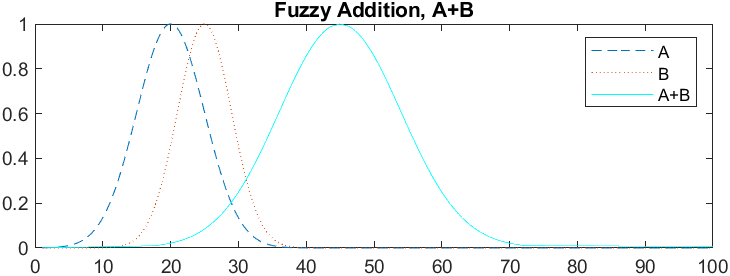
\includegraphics[scale=1]{addition.png}
    \caption{\label{fig:add_img} Graphs of $\mu_{\Tilde{A}}(x) \:=\:e^{\left( \frac{-(x-20)^2}{2(5)^{2}} \right)}$, $\mu_{\Tilde{B}}(x) \:=\:e^{\left( \frac{-(x-25)^2}{2(4)^{2}} \right)}$, and $\mu_{\Tilde{A}\oplus\Tilde{B}}(x) \:=\:e^{\left( \frac{-(x-45)^2}{2(9)^{2}}\right)}$}
    \label{fig:add_img}
\end{figure}

\subsection{Subtraction of Gaussian Fuzzy Numbers}
Consider two fuzzy numbers $\Tilde{A}$ and $\Tilde{B}$ defined on $\mathbb{R}$, with membership functions given by:
\[ \mu_{\Tilde{A}}(x) \:=\:e^{\left[ \frac{-(x-m_{\Tilde{A}})^2}{2\sigma_{\Tilde{A}}^{2}} \right]}\;  ; \;\mu_{\Tilde{B}}(x) \: = \:e^{\left[ \frac{-(x-m_{\Tilde{B}})^2}{2\sigma_{\Tilde{B}}^{2}} \right]} \]
The $\alpha$-cuts for $\Tilde{A}$ and $\Tilde{B}$ are: \[ \Tilde{A}_{\alpha} = \left[m_{\Tilde{A}}-\sigma_{\Tilde{A}}\sqrt{-2\ln{\alpha}}, \: m_{\Tilde{A}}+\sigma_{\Tilde{A}}\sqrt{-2\ln{\alpha}} \right]\] and, \[ \Tilde{B}_{\alpha} = \left[m_{\Tilde{B}}-\sigma_{\Tilde{B}}\sqrt{-2\ln{\alpha}}, \: m_{\Tilde{B}}+\sigma_{\Tilde{B}}\sqrt{-2\ln{\alpha}} \right]\] respectively, for $\alpha\in(0,1]$. Upon interval subtraction of $\alpha$-cuts of $\Tilde{A}$ and $\Tilde{B}$, we get:
\begin{equation}\label{subexp}
 (\Tilde{A}\ominus\Tilde{B})_\alpha\,=\, \Tilde{A}_\alpha \: - \: \Tilde{B}_\alpha = \left[(m_{\Tilde{A}}\, - \, m_{\Tilde{B}})-(\sigma_{\Tilde{A}}+\sigma_{\Tilde{B}})\sqrt{-2\ln{\alpha}}, \: (m_{\Tilde{A}}\, - \, m_{\Tilde{B}})+(\sigma_{\Tilde{A}}+\sigma_{\Tilde{B}})\sqrt{-2\ln{\alpha}}\right] ; \quad\alpha\in [0,1]  
\end{equation} \newline By comparing (\ref{subexp}) to $alpha$-cut of a Gaussian fuzzy number given by (\ref{alpha_fuzzy}), we get:
\begin{equation}
    \sigma_{\Tilde{A}\ominus\Tilde{B}} = \sigma_{\Tilde{A}} - \sigma_{\Tilde{B}}, \quad m_{\Tilde{A}\ominus\Tilde{B}} = m_{\Tilde{A}} - m_{\Tilde{B}}, \quad 
    \mu_{\Tilde{A}\ominus\Tilde{B}}(x) \,=\, e^{\left[ \frac{-(x-(m_{\Tilde{A}} - m_{\Tilde{B}} ))^2}{2(\sigma_{\Tilde{A}} + \sigma_{\Tilde{B}} )^{2}} \right]};\: \forall x \,\in\, \mathbb{R}
\end{equation}
\newline
\textbf{Example} : Let $\Tilde{A}$ and $\Tilde{B}$ be two Gaussian fuzzy numbers defined on $\mathbb{R}$ with $\sigma_{\Tilde{A}} = 5, \:m_{\Tilde{A}} = 20$; and $\sigma_{\Tilde{B}} = 4, \:m_{\Tilde{B}} = 25$ respectively. We get membership functions of $\Tilde{A}$ and $\Tilde{B}$ as $\mu_{\Tilde{A}}(x) \:=\:e^{\left( \frac{-(x-20)^2}{2(5)^{2}} \right)}$ and $\mu_{\Tilde{B}}(x) \:=\:e^{\left( \frac{-(x-25)^2}{2(4)^{2}} \right)}$. On addition of $\Tilde{A}$ and $\Tilde{B}$, we get $\mu_{\Tilde{A}\ominus\Tilde{B}}(x) \:=\:e^{\left( \frac{-(x+5)^2}{2(9)^{2}}\right)}$. Figure \ref{fig:sub_img} shows MATLAB plots of $\Tilde{A}$, $\Tilde{B}$ and $\Tilde{A}\ominus\Tilde{B}$.

\begin{figure}[h!]
    \centering
    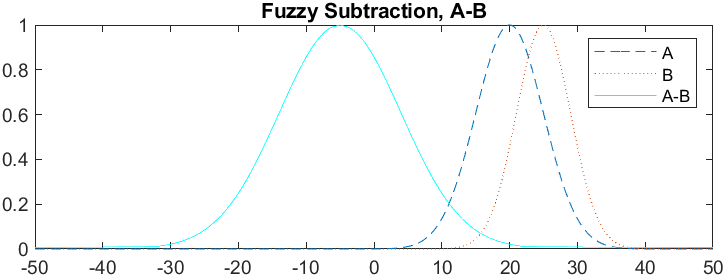
\includegraphics[scale=1]{subtraction.png}
    \caption{\label{fig:sub_img} Graphs of $\mu_{\Tilde{A}}(x) \:=\:e^{\left( \frac{-(x-20)^2}{2(5)^{2}} \right)}$, $\mu_{\Tilde{B}}(x) \:=\:e^{\left( \frac{-(x-25)^2}{2(4)^{2}} \right)}$, and $\mu_{\Tilde{A}\ominus\Tilde{B}}(x) \:=\:e^{\left( \frac{-(x+5)^2}{2(9)^{2}}\right)}$}
    \label{fig:sub_img}
\end{figure}

\subsection{Multiplication of Gaussian Fuzzy Numbers}
Consider two Gaussian fuzzy numbers $\Tilde{A} \,=\, \left(m_{\Tilde{A}},\: \sigma_{\Tilde{A}}, \:\sigma_{\Tilde{A}}\right)_{L,R}$ and $\Tilde{B}\,=\, \left(m_{\Tilde{B}},\: \sigma_{\Tilde{B}}, \:\sigma_{\Tilde{B}}\right)_{L,R}$, defined on $\mathbb{R}$ with $L(u) \,=\, R(u)\,=\,e^{\frac{-u^2}{2}}\implies L^{-1}(u) = R^{-1} (u) = \sqrt{-2\ln{x}}$. The membership functions of $\Tilde{A}$ and $\Tilde{B}$ given by:
\[ \mu_{\Tilde{A}}(x) \:=\:e^{\left[ \frac{-(x-m_{\Tilde{A}})^2}{2\sigma_{\Tilde{A}}^{2}} \right]}\;  ; \;\mu_{\Tilde{B}}(x) \: = \:e^{\left[ \frac{-(x-m_{\Tilde{B}})^2}{2\sigma_{\Tilde{B}}^{2}} \right]} \forall x\in \mathbb{R} \] 
The $\alpha$-cuts for $\Tilde{A}$ and $\Tilde{B}$ are: \[ \Tilde{A}_{\alpha} = \left[m_{\Tilde{A}}-\sigma_{\Tilde{A}}\sqrt{-2\ln{\alpha}}, \: m_{\Tilde{A}}+\sigma_{\Tilde{A}}\sqrt{-2\ln{\alpha}} \right]\] and, \[ \Tilde{B}_{\alpha} = \left[m_{\Tilde{B}}-\sigma_{\Tilde{B}}\sqrt{-2\ln{\alpha}}, \: m_{\Tilde{B}}+\sigma_{\Tilde{B}}\sqrt{-2\ln{\alpha}} \right]\] respectively, for $\alpha\in[0,1]$.
\[
\text{Let}\quad a\: = \:m_{\Tilde{A}}-\sigma_{\Tilde{A}}\sqrt{-2\ln{\alpha}},\] 
\[b \: =  \: m_{\Tilde{A}}+\sigma_{\Tilde{A}}\sqrt{-2\ln{\alpha}},\]
\[c \: =\: m_{\Tilde{B}}-\sigma_{\Tilde{B}}\sqrt{-2\ln{\alpha}}, \]
\[d = \: m_{\Tilde{B}}+\sigma_{\Tilde{B}}\sqrt{-2\ln{\alpha}}.
\]\newline Upon interval multiplication of $\alpha$-cuts, we get:
\begin{equation}\label{mulexp}
 (\Tilde{A}\otimes\Tilde{B})_\alpha\,=\,\Tilde{A}_\alpha \: \times \: \Tilde{B}_\alpha = \left[ \text{min}\left\{ac, ad, bc, bd \right\}, \text{max}\left\{ac, ad, bc, bd \right\} \right]  
\end{equation}\newline If we try to calculate the exact value of the membership function using equation (\ref{mulexp}), the resulting fuzzy number may not be a Gaussian fuzzy number. The exact interval of the $\alpha$-cut in equation (\ref{mulexp}) depends upon the signs of $a$, $b$, $c$, $d$, which give rise to various cases. Let us consider the case where $\Tilde{A} > 0$, (i.e., $m_{\Tilde{A}} > 0,\; m_{\Tilde{A}} - \sigma_{\Tilde{A}} >0,\; m_{\Tilde{A}} + \sigma_{\Tilde{A}} > 0$, so, $\mu_{\Tilde{A}}\approx0\; \forall x\leq0$) and similarly, $\Tilde{B} > 0$. From equation (\ref{mulexp}), we get:
\begin{equation}\label{mulalp}
(\Tilde{A}\otimes\Tilde{B})_\alpha\,=\,\Tilde{A}_\alpha \: \times \: \Tilde{B}_\alpha = \left[ 
\left(m_{\Tilde{A}}-\sigma_{\Tilde{A}}\sqrt{-2\ln{\alpha}}\right)\left(m_{\Tilde{B}}-\sigma_{\Tilde{B}}\sqrt{-2\ln{\alpha}}\right), \; \left( m_{\Tilde{A}}+\sigma_{\Tilde{A}}\sqrt{-2\ln{\alpha}}\right)\left(m_{\Tilde{B}}+\sigma_{\Tilde{B}}\sqrt{-2\ln{\alpha}}\right)\right]\end{equation}\[\quad\alpha\in [0,1]\]\newline On simplification and using tangent approximation on equation (\ref{mulalp}), we get:
\begin{equation}
\Tilde{A}\otimes\Tilde{B} \approx \left(m_{\Tilde{A}}m_{\Tilde{B}},\; m_{\Tilde{A}}\sigma_{\Tilde{B}}+m_{\Tilde{B}}\sigma_{\Tilde{A}},\; m_{\Tilde{A}}\sigma_{\Tilde{B}}+m_{\Tilde{B}}\sigma_{\Tilde{A}} \right)_{L,R}\quad;\;\newline L(u) = R(u) = e^{\frac{-u^2}{2}}   \forall u\in \mathbb{R}
\end{equation}\newline Similarly, on simplification and secant approximation, we get:
\begin{equation}
\Tilde{A}\otimes\Tilde{B} \approx \left(m_{\Tilde{A}}m_{\Tilde{B}},\; m_{\Tilde{A}}\sigma_{\Tilde{B}}+m_{\Tilde{B}}\sigma_{\Tilde{A}} + \sigma_{\Tilde{A}}\sigma_{\Tilde{B}},\; m_{\Tilde{A}}\sigma_{\Tilde{B}}+m_{\Tilde{B}}\sigma_{\Tilde{A}}+\sigma_{\Tilde{A}}\sigma_{\Tilde{B}} \right)_{L,R}\quad;\; L(u) = R(u) = e^{\frac{-u^2}{2}}   
\end{equation}\newline Figure (\ref{fig:prod_img}) shows the multiplication of two Gaussian fuzzy numbers $\Tilde{A} = \left(5,1,1\right)_{L,R}$ and $\Tilde{B} = \left(5,2,2\right)_{L,R}$ with $L(u) = R(u) = e^{\frac{-u^2}{2}} \; \forall u\in\mathbb{R}$.

\begin{figure}
    \centering
    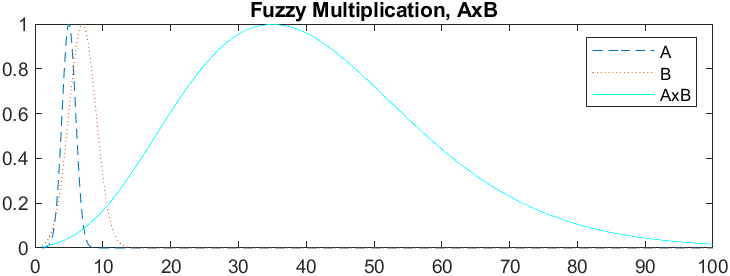
\includegraphics[scale=1]{multiplication.png}
    \caption{\label{fig:prod_img} Graphs of $\mu_{\Tilde{A}}(x) \:=\:e^{\left( \frac{-(x-5)^2}{2(1)^{2}} \right)}$, $\mu_{\Tilde{B}}(x) \:=\:e^{\left( \frac{-(x-7)^2}{2(2)^{2}} \right)}$, and $\mu_{\Tilde{A}\otimes\Tilde{B}}(x)$}
    \label{fig:prod_img}
\end{figure}


\subsection{Reciprocal of Gaussian Fuzzy Number}
Consider a Gaussian fuzzy number $\Tilde{A} \,=\, \left(m,\: \sigma, \:\sigma\right)_{L,R}$ on $\mathbb{R}$ with $L(u) \,=\, R(u)\,=\,e^{\frac{-u^2}{2}}\implies L^{-1}(u) = R^{-1} (u) = \sqrt{-2\ln{x}}$. For a Gaussian Fuzzy number, the value of membership is not 0 at $x = 0$. So, reciprocal is not defined for a Gaussian fuzzy number. But, if we assume that $m>0,\; \sigma + m>0 '\; m-\sigma>0$ or $m<0,\; \sigma + m <0,\; m-\sigma <0$, the Gaussian fuzzy number approximately lies entirely on one side of $x = 0$. In such a case, $\mu_{\Tilde{A}}(0)\approx0$. So, we can neglect the membership function at $x = 0$. To calculate the approximate value of the reciprocal of Gaussian Fuzzy Number $\Tilde{A}$, we use tangent and secant approximation. Using tangent approximation, we get:
\begin{equation}
    \left(\Tilde{A}^{-1}\right)_t \,=\, \left(\frac{1}{m}, \frac{\sigma}{{m}^2}, \frac{\sigma}{{m}^2}\right)_{R,L} \, \approx\, \Tilde{A}^{-1}\; 
\end{equation}\newline Using secant approximation, we get:
\begin{equation}
    \left(\Tilde{A}^{-1}\right)_s \,=\, \left(\frac{1}{m}, \frac{\sigma}{m(m + \sigma)}, \frac{\sigma}{m(m - \sigma)}\right)_{R,L} \, \approx\, \Tilde{A}^{-1}\; 
\end{equation} 

\subsection{Division of Gaussian Fuzzy Numbers}
Consider two Gaussian fuzzy numbers $\Tilde{A} \,=\, \left(m_{\Tilde{A}},\: \sigma_{\Tilde{A}}, \:\sigma_{\Tilde{A}}\right)_{L,R}$ and $\Tilde{B}\,=\, \left(m_{\Tilde{B}},\: \sigma_{\Tilde{B}}, \:\sigma_{\Tilde{B}}\right)_{L,R}$, defined on $\mathbb{R}$ with $L(u) \,=\, R(u)\,=\,e^{\frac{-u^2}{2}}\implies L^{-1}(u) = R^{-1} (u) = \sqrt{-2\ln{x}}$. The membership functions of $\Tilde{A}$ and $\Tilde{B}$ given by:
\[ \mu_{\Tilde{A}}(x) \:=\:e^{\left[ \frac{-(x-m_{\Tilde{A}})^2}{2\sigma_{\Tilde{A}}^{2}} \right]}\;  ; \;\mu_{\Tilde{B}}(x) \: = \:e^{\left[ \frac{-(x-m_{\Tilde{B}})^2}{2\sigma_{\Tilde{B}}^{2}} \right]} \]
The $\alpha$-cuts for $\Tilde{A}$ and $\Tilde{B}$ are: \[ \Tilde{A}_{\alpha} = \left[m_{\Tilde{A}}-\sigma_{\Tilde{A}}\sqrt{-2\ln{\alpha}}, \: m_{\Tilde{A}}+\sigma_{\Tilde{A}}\sqrt{-2\ln{\alpha}} \right]\] and, \[ \Tilde{B}_{\alpha} = \left[m_{\Tilde{B}}-\sigma_{\Tilde{B}}\sqrt{-2\ln{\alpha}}, \: m_{\Tilde{B}}+\sigma_{\Tilde{B}}\sqrt{-2\ln{\alpha}} \right]\] respectively, for $\alpha\in[0,1]$.
\[
\text{Let}\quad a\: = \:m_{\Tilde{A}}-\sigma_{\Tilde{A}}\sqrt{-2\ln{\alpha}},\] 
\[b \: =  \: m_{\Tilde{A}}+\sigma_{\Tilde{A}}\sqrt{-2\ln{\alpha}},\]
\[c \: =\: m_{\Tilde{B}}-\sigma_{\Tilde{B}}\sqrt{-2\ln{\alpha}}, \]
\[d = \:  m_{\Tilde{B}}+\sigma_{\Tilde{B}}\sqrt{-2\ln{\alpha}}.
\]\newline Upon interval division of $\alpha$-cuts, we get:
\begin{equation}\label{divexp}
 (\Tilde{A}\oslash\Tilde{B})_\alpha\,=\,\Tilde{A}_\alpha \: / \: \Tilde{B}_\alpha = \left[ \text{min}\left\{a/c, a/d, b/c, b/d \right\}, \text{max}\left\{a/c, a/d, b/c, b/d \right\} \right]; \quad\alpha\in [0,1]
\end{equation}\newline Similar to what was seen while calculating the reciprocal of a Gaussian Fuzzy number, division of two Gaussian Fuzzy numbers is not defined, since the value of the membership function of the denominator at $x=0$ is not zero. But, if we assume that for the Gaussian fuzzy number $\Tilde{B}$ in the denominator,  $m_{\Tilde{B}}>0,\; \sigma_{\Tilde{B}} + m_{\Tilde{B}}>0 '\; m_{\Tilde{B}}-\sigma_{\Tilde{B}}>0$ or $m_{\Tilde{B}}<0,\; \sigma_{\Tilde{B}} + m_{\Tilde{B}} <0,\; m_{\Tilde{B}}-\sigma_{\Tilde{B}} <0$, the Gaussian fuzzy number approximately lies entirely on one side of $x = 0$. In such a case, $\mu_{\Tilde{B}}(0)\approx0$. So, we can neglect the value of the membership function of the denominator $\Tilde{B}$ at $x = 0$. Still, calculating the exact curve of equation (\ref{divexp}) would be complicated. So we use use tangent and secant approximation and multiply $\Tilde{A}$ with the reciprocal $\Tilde{1/B}$ to get the approximate result of division.
\begin{equation}
    \Tilde{A}\oslash\Tilde{B}\,=\,\Tilde{A} \times1/\Tilde{B}
\end{equation}\newline Figure (\ref{fig:div_img}) shows the division of two Gaussian fuzzy numbers $\Tilde{A} = \left(40,4,4\right)_{L,R}$ by $\Tilde{B} = \left(8,2,2\right)_{L,R}$ with $L(u) = R(u) = e^{\frac{-u^2}{2}} \; \forall u\in\mathbb{R}$.


\begin{figure}
    \centering
    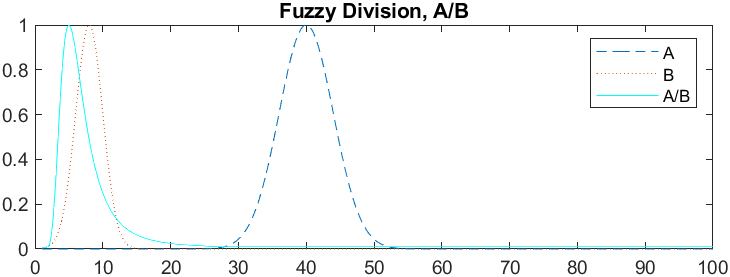
\includegraphics[scale=1]{division.png}
    \caption{\label{fig:div_img} Graphs of $\mu_{\Tilde{A}}(x) \:=\:e^{\left( \frac{-(x-40)^2}{2(4)^{2}} \right)}$, $\mu_{\Tilde{B}}(x) \:=\:e^{\left( \frac{-(x-8)^2}{2(2)^{2}} \right)}$, and $\mu_{\Tilde{A}\oslash\Tilde{B}}(x)$}
    \label{fig:div_img}
\end{figure}


\subsection{Exponent of a Gaussian Fuzzy Number}\
Consider Gaussian fuzzy number $\Tilde{A}$ with mean $m$  and standard deviation $\sigma_{\Tilde{A}}$.\newline $\alpha$-cut of $\Tilde{A}$ is $\Tilde{A}_\alpha \: = \: \left[m_{\Tilde{A}}-\sigma_{\Tilde{A}}\sqrt{-2\ln{\alpha}}, \: m_{\Tilde{A}}+\sigma_{\Tilde{A}}\sqrt{-2\ln{\alpha}} \right]$.\newline 
To calculate exp($\Tilde{A}$) or $e^{(\Tilde{A})}$ we first take the exponent of the $\alpha$-cut.
\[(exp(\Tilde{A}))_\alpha = exp(\Tilde{A}_\alpha)=[exp(m_{\Tilde{A}}-\sigma_{\Tilde{A}}\sqrt{-2\ln{\alpha}}),exp(m_{\Tilde{A}}+\sigma_{\Tilde{A}}\sqrt{-2\ln{\alpha}})]\quad\alpha\in [0,1]\]
The next step is to fuzzify the obtained interval. Let
\[x=exp(m_{\Tilde{A}}-\sigma_{\Tilde{A}}\sqrt{-2\ln{\alpha}})\]
\[\ln{x}=m_{\Tilde{A}}-\sigma_{\Tilde{A}}\sqrt{-2\ln{\alpha}}\]
\[\ln{\alpha}=\frac{-1}{2}\biggl({\frac{m_{\Tilde{A}}-\ln{x}}{\sigma_{\Tilde{A}}}}\biggr)^2\]
\[\alpha=exp\biggl(\frac{-1}{2}\biggl({\frac{m_{\Tilde{A}}-\ln{x}}{\sigma_{\Tilde{A}}}}\biggr)^2\biggr)\quad ;\quad 0 < x\leq exp(m_{\Tilde{A}})\]
Similarly, for the right interval value, we get, 
\[\alpha=exp\biggl(\frac{-1}{2}\biggl({\frac{- m_{\Tilde{A}}+\ln{x}}{\sigma_{\Tilde{A}}}}\biggr)^2\biggr)\quad ;\quad x\geq exp(m_{\Tilde{A}})\]
Therefore,
\[e^{\Tilde{A}}=\begin{cases}
        exp\biggl(\frac{-1}{2}\biggl({\frac{m_{\Tilde{A}}-\ln{x}}{\sigma_{\Tilde{A}}}}\biggr)^2\biggr)& \text{if } x > 0\\
        0 & \text{elsewhere } 
        \end{cases}\]

\textbf{Example} : Let $\Tilde{A}$ be a Gaussian fuzzy number defined on $\mathbb{R}$ with $\sigma_{\Tilde{A}} = 1, \:m_{\Tilde{A}} = 5$. We get membership function of $\Tilde{A}$  as $\mu_{\Tilde{A}}(x) \:=\:e^{\left( \frac{-(x-5)^2}{2(1)^{2}} \right)}$ . On exponentiation of $\Tilde{A}$, we get $\mu_{e^{\Tilde{A}}}=exp\biggl(\frac{-1}{2}\biggl({\frac{5-\ln{x}}{1}}\biggr)^2\quad ;\quad x > 0 $. Figure \ref{fig:e_img} shows  plots of $\Tilde{A}$ and $e^{\Tilde{A}}$.
% \subsection{How to add Tables}

% Use the table and tabular environments for basic tables --- see Table~\ref{tab:widgets}, for example. For more information, please see this help article on \href{https://www.overleaf.com/learn/latex/tables}{tables}. 

% \begin{table}
% \centering
% \begin{tabular}{l|r}
% Item & Quantity \\\hline
% Widgets & 42 \\
% Gadgets & 13
% \end{tabular}
% \caption{\label{tab:widgets}An example table.}
% \end{table}
\begin{figure}[h!]
    \centering
    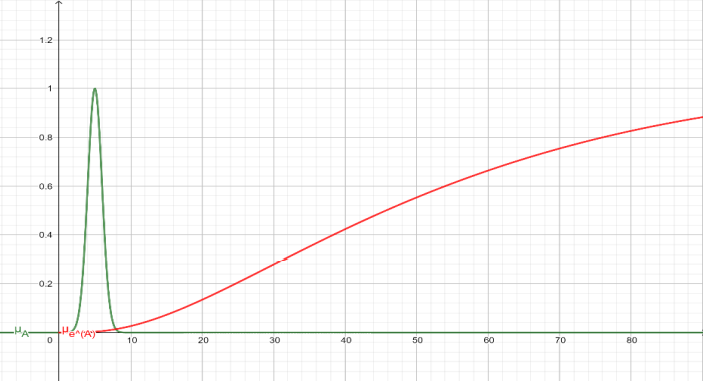
\includegraphics[scale=0.7]{gaussian_e.png}
    \caption{\label{fig:e_img} Graphs of $\mu_{\Tilde{A}}(x) \:=\:e^{\left( \frac{-(x-5)^2}{2(1)^{2}} \right)}$, and $\mu_{ln({\Tilde{A}})}=exp\biggl(\frac{-1}{2}\biggl({\frac{5-ln({x})}{1}}\biggr)^2\biggr)$}
    
    \label{fig:e_img}
\end{figure}

\subsection{Natural Logarithm of Gaussian Fuzzy number}
Consider Gaussian fuzzy number $\Tilde{A}$ with mean $m$  and standard deviation $\sigma_{\Tilde{A}}$.\newline $\alpha$-cut of $\Tilde{A}$ is $\Tilde{A}_\alpha \: = \: \left[m_{\Tilde{A}}-\sigma_{\Tilde{A}}\sqrt{-2\ln{\alpha}}, \: m_{\Tilde{A}}+\sigma_{\Tilde{A}}\sqrt{-2\ln{\alpha}} \right]$.\newline 
To calculate ln($\Tilde{A}$)  we first take the natural logarithm of the $\alpha$-cut.
\[(ln(\Tilde{A}))_\alpha = ln(\Tilde{A}_\alpha)=[ln(m_{\Tilde{A}}-\sigma_{\Tilde{A}}\sqrt{-2\ln{\alpha}}),ln(m_{\Tilde{A}}+\sigma_{\Tilde{A}}\sqrt{-2\ln{\alpha}})]\quad\alpha\in [0,1]\]
The next step is to fuzzify the obtained interval. Let
\[x=ln(m_{\Tilde{A}}-\sigma_{\Tilde{A}}\sqrt{-2\ln{\alpha}})\]
\[e^{x}=m_{\Tilde{A}}-\sigma_{\Tilde{A}}\sqrt{-2\ln{\alpha}}\]
\[\ln{\alpha}=\frac{-1}{2}\biggl({\frac{m_{\Tilde{A}}- e^{x}}{\sigma_{\Tilde{A}}}}\biggr)^2\]
\[\alpha=exp\biggl(\frac{-1}{2}\biggl({\frac{m_{\Tilde{A}}-e^{x}}{\sigma_{\Tilde{A}}}}\biggr)^2)\quad ;\quad \forall x\in\mathbb{R}\]
We get,
\[ln({\Tilde{A}})=\begin{cases}
        exp\biggl(\frac{-1}{2}\biggl({\frac{m_{\Tilde{A}}- e^{x}}{\sigma_{\Tilde{A}}}}\biggr)^2\biggr)& \forall x \in \mathbb{R}\\
     
        \end{cases}\]
\textbf{Example} : Let $\Tilde{A}$ be a Gaussian fuzzy number defined on $\mathbb{R}$ with $\sigma_{\Tilde{A}} = 1, \:m_{\Tilde{A}} = 10$. We get membership function of $\Tilde{A}$  as $\mu_{\Tilde{A}}(x) \:=\:e^{\left( \frac{-(x-10)^2}{2(1)^{2}} \right)}$ . On taking logarithm of $\Tilde{A}$, we get $\mu_{ln({\Tilde{A}})}=exp\biggl(\frac{-1}{2}\biggl({\frac{10-e^{x}}{1}}\biggr)^2\biggr)\quad \forall x \in \mathbb{R} $. Figure \ref{fig:ln_img} shows plots of $\Tilde{A}$ and $ln(\Tilde{A})$.

\vspace{3cm}

\begin{figure}[h]
    \centering
    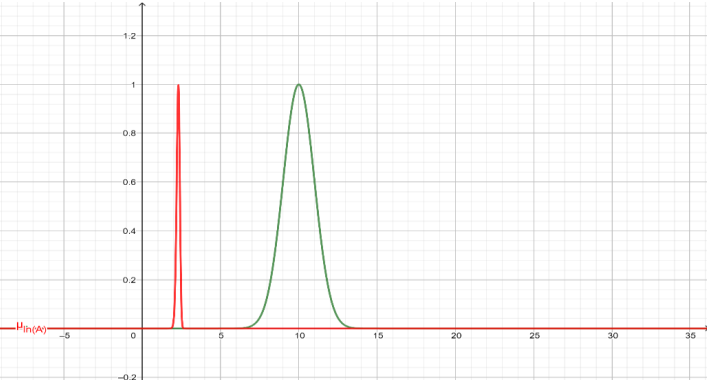
\includegraphics[scale=0.7]{gaussian_ln.png}
    \caption{\label{fig:ln_img} Graphs of $\mu_{\Tilde{A}}(x) \:=\:e^{\left( \frac{-(x-10)^2}{2(1)^{2}} \right)}$, and $\mu_{ln({\Tilde{A}})}=exp\biggl(\frac{-1}{2}\biggl({\frac{10-e^{x}}{1}}\biggr)^2\biggr)$}
    
    \label{fig:ln_img}
\end{figure}
\section{Conclusion}
In this paper, we have discussed the definiton of the Gaussian Fuzzy Number and also shown its representation using the L-R Fuzzy Number. We have used the $\alpha$-cut method to evalutate various arithmetic operations on the Gaussian fuzzy number.
\bibliographystyle{alpha}
\bibliography{sample}

\end{document}